\documentclass[11pt,a4paper]{article}
\usepackage[utf8]{inputenc}
\usepackage[spanish]{babel}
\usepackage{biblatex}
\usepackage{amssymb, amsmath, amsbsy}
\usepackage{graphicx}
\usepackage{makeidx}
\usepackage{color,xcolor}
\usepackage[left=2cm,right=2cm,top=2cm,bottom=2cm]{geometry}
\usepackage[linkcolor=black,colorlinks=true,urlcolor=blue]{hyperref}
\usepackage{xcolor}
\usepackage{fancyhdr}
\usepackage{float}
\usepackage{subfigure}
\renewcommand{\baselinestretch}{1.5}
\addbibresource{bib.bib}
\setlength{\parindent}{0em}
\bibliography{bib}

\begin{document}

\thispagestyle{empty}
\begin{center}

\includegraphics[width=10cm]{logo udesa.PNG}
\end{center}


	\begin{center}
	\LARGE
	Herramientas Computaciones para Investigación
\\			\vspace{1cm}
\hrule
	\vspace{0.5cm}
	\LARGE
 Tema 3 - Python Scrapping
\\		
		\vspace{0.5cm}
		\hrule
				\vspace{1cm}
	\large

	\vspace{2.5cm}
	\large
		Alumnos:\\
	\large
	Elard Amaya, Francisco Guerrero
	
	
	\vspace{1.3cm}
	\normalsize	
	Profesora:\\

	\normalsize
	Amelia Gibbons
	
	\vspace{1.3cm}
	\today
	\end{center}

\clearpage
\section*{Parte 1 - Precipitaciones y crímenes}

En la primera parte del trabajo, exploramos si existe alguna asociación entre el nivel de precipitaciones y la ocurrencia de hurtos en los condados de Maryland (Figura 1). Agregamos los datos en indicadores anuales, con la finalidad de mostrar asociaciones más claras entre dichas variables. En el Panel a, usamos la ocurrencia de hurtos anuales per-cápita y el nivel de precipitaciones anuales, para la construcción de ambos indicadores realizamos un agregado de lo reportado mensualmente. Por su parte, en el Panel b, usamos la ocurrencia promedio mensual de hurtos per-cápita y el nivel promedio mensual de precipitaciones, para estos indicadores empleamos el promedio de lo reportado mensualmente.\footnote{Utilizamos el siguente comando en la ventana de QGIS para el calculo de los hurtos totales y promedio:
\emph{sum((Theft/POPULATION),FIPS)/count(CNTY\_FI,FIPS)}, para hurtos totales eliminamos la función \emph{count} y para hurtos promedio se divide entre la cantidad de meses sin valores missing. Para precipitaciones hacemos lo mismo.}
\\
Ambos gráficos aparentan mostrar una correlación positiva entre la ocurrencia de hurtos y el nivel de precipitaciones. La literatura que ha explorado la asociación clima-crimen ha sido concluyente respecto a que la exposición a climas extremos tiene un impacto sobre los crímenes a la propiedad y crímenes violentos, principalmente la exposición a shocks climáticos calurosos \cite{blakeslee_weather_2018,cohn_weather_1990,trujillo_effect_2021}. Para el caso de shocks de lluvia y crimen, la literatura ha mostrado resultados mixtos \cite{blakeslee_weather_2018,field_effect_1992,schutte_influence_2018}, basándose en dos mecanismos. Primero, las lluvias son escenarios favorales para los criminales, al hacer más complicado el patrullaje y en consecuencia el resguardo policial. Por otro lado, las lluvias en grandes dimensiones reducen el tránsito cotidiano de la gente en las calles, por lo que los escenarios de contacto entre víctimas y agresores es menor y en consecuencia las oportunidades de robo también \cite{field_effect_1992}. Estos mecanismos en conjunto hacen menos evidente conocer el efecto conjunto de las lluvias sobre la criminalidad. Todo lo anterior, sugiere que la asociación preliminar encontrada aun requiere de mayor exploración.


\begin{figure}[!h]
    \centering
    \subfigure[]{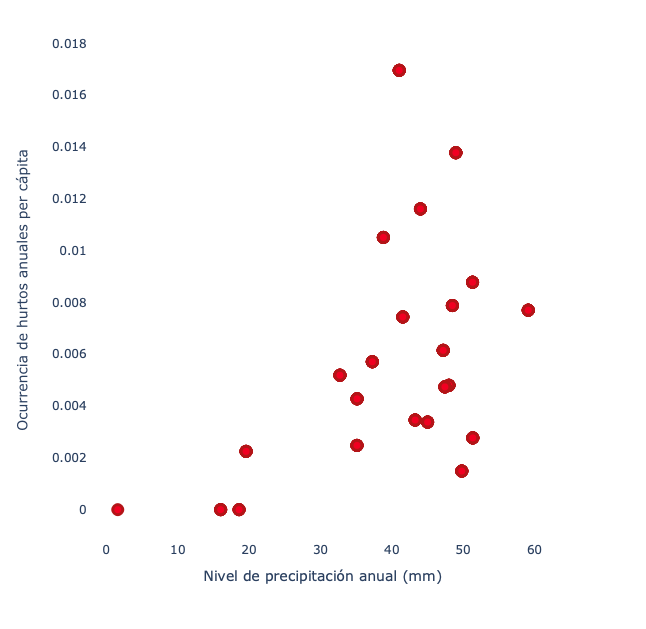
\includegraphics[width=6.5cm]{Graph/part1 graph1.png}}
    \subfigure[]{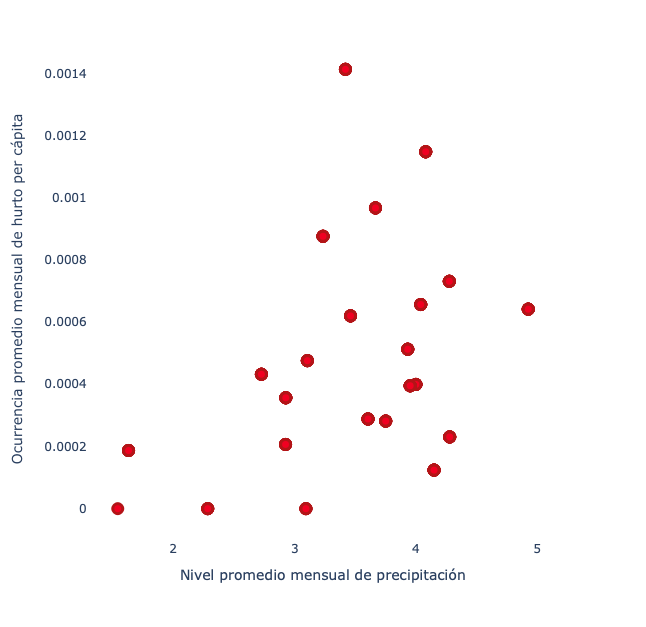
\includegraphics[width=6.5cm]{Graph/part1 graph2.png}}
    \caption{Relación entre hurtos y precipitaciones, condados de Maryland - 2015}
    \label{fig:my_label}
\end{figure}


\clearpage
\section*{Parte 2 - Datos de Afroamericanos}

En la segunda parte del trabajo, exploramos la asociación que podría existir entre la proporción de afroamericanos y la cantidad de crímenes en los condados de Maryland (Figura 2); calculamos la ocurrencia de crímenes anual agregando los tipos de crímenes y su ocurrencia mensual.\footnote{Utilizamos el siguiente comando en la ventana de QGIS para agregar los crímenes: \emph{sum((Robbery+Assault+Theft+BrkngE\_)/POPULAT),FIPS)*10000)}}
\\
El motivo de esta exploración es que en Estados Unidos se tiene la creencia popular de que las zonas más habitadas por afroamericanos son las más propensas al crimen y la violencia \cite{wolfgang_crime_1964}, creencia que se estimula por las mayores detenciones y sentencias contra los afroamericanos, las cuales siguen criterios sesgados que refuerzan estos estereotipos \cite{steffensmeier_ethnicity_2000,weitzer_race_2004}. Nuestro gráfico de dispersión se corresponde hasta cierto punto con esta creencia, sin embargo, no es posible validarla dado que encontramos condados con indices de crimen bastante bajos donde más de la mitad de la población habitante es afroamericana. A su vez, cabe mencionar que estos condados donde no se cumple dicha creencia son aquellos con la mayor población en el estado de Maryland.
\\
Elaborar este tipo de relaciones bifactoriales entre grupos étnicos y ocurrencia de crimen no es lo adecuado, dado que la ocurrencia del crimen no tiene un origen unidimensional, sino que incurren diversos factores tales como el desempleo, la desigualdad, la discriminación, entre otros; y centrar su causa en un grupo étnico ignora los problemas estructurales que ocasionan el crimen, y en consecuencia, vuelven más difícil enfrentar la criminalidad.

\begin{figure}[!h]
    \centering
    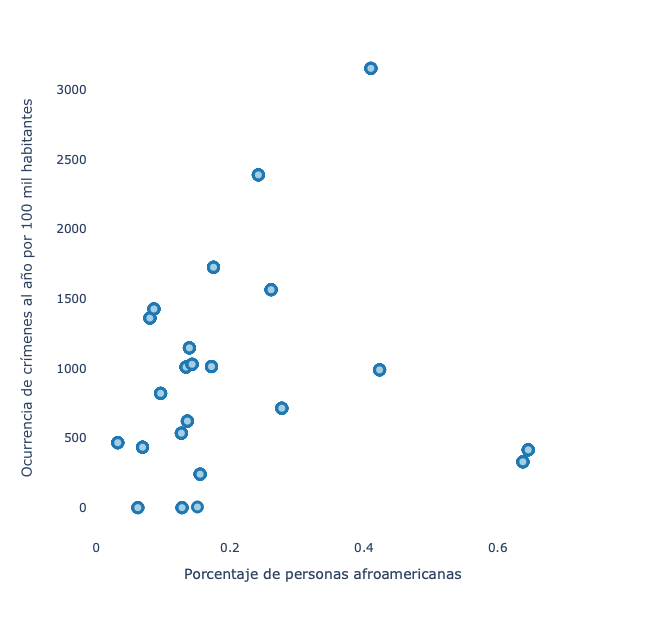
\includegraphics[width=10cm]{Graph/part2 graph1.png}
   \caption{Proporción de afroamericanos y ocurrencia de crimenes, Condados de Maryland - 2015}
    \label{fig:my_label}
\end{figure}

\clearpage
\printbibliography

\end{document}
